%%%%%%%%%%%%%%%%%%%%%%%%%%%%%%%%%%%%%%%%%%%%%%%%%%%%%%%%%%%%%%%%%%%%%%%%%%%%%%%%%
%																				%
%	TRABAJO:	Trabajo Final													%
%				Especialidad en Ingenier�a en Sistemas de Informaci�n			%
%																				%
%		Titulo:																	%
%																				%
%		Autores:	Julian Nonino												%
%																				%
%	DOCUMENTO PRINCIPAL															%	
%																				%
%	A�o: 2016																	%
%																				%
%%%%%%%%%%%%%%%%%%%%%%%%%%%%%%%%%%%%%%%%%%%%%%%%%%%%%%%%%%%%%%%%%%%%%%%%%%%%%%%%%

\documentclass[a4paper,12pt,openright,twoside]{book}

% Paquetes
	% Idioma y codificacion de caracteres
		\usepackage[spanish]{babel}
		\usepackage[latin1]{inputenc}
	% Figuras
		\usepackage{graphicx}
		\usepackage{subfigure}
		\usepackage{float} % Para posicionar imagenes donde uno quiera. Solo hay que poner la opcion [H]
	% Apendice
		\usepackage{appendix}
	%Tablas	
	%\usepackage{tabular}
	% Margenes
		\usepackage{anysize}
	% Tabla de conteido
		\usepackage[tight]{shorttoc}
	% Matematica
		\usepackage[cmex10]{amsmath}
		\usepackage{amssymb}
	% Colores
		\usepackage{color}
		% Definicion de colores
			\definecolor{dkgreen}{rgb}{0,0.6,0}
			\definecolor{gray}{rgb}{0.5,0.5,0.5}
			\definecolor{mauve}{rgb}{0.58,0,0.82}
			\definecolor{violeta}{RGB}{127,0,85}
	% Insertar c�digo
		\usepackage{listings}
	% URLs
		\usepackage{url}
	% Referencias
		%\usepackage[dcucite]{harvard}
		\usepackage{hyperref}
		\usepackage[style=numeric,backend=bibtex]{biblatex}
		\addbibresource{referencias.bib}

% Margenes
	% Controla los m�rgenes {izquierda}{derecha}{arriba}{abajo}
		\marginsize{3cm}{3cm}{2.5cm}{2.5cm}

% Encabezados
	\pagestyle{headings}
		
% Documento
\begin{document}
 
	% Reeescritura de comandos
		\renewcommand{\appendixname}{Ap�ndice}
		\renewcommand{\appendixtocname}{Ap�ndice}
		\renewcommand{\tablename}{\textbf{Tabla}} 	% Para poner la palabra en mayusucula
		\renewcommand{\figurename}{\textbf{Figura}} % Para poner la palabra en mayuscula
		\renewcommand{\contentsname}{�ndice}
		\renewcommand{\listtablename}{�ndice de tablas}
		\renewcommand{\listfigurename}{�ndice de Figuras}

		\setcounter{secnumdepth}{3} % Para numerar subsubsecciones
		\setcounter{tocdepth}{3}	% Para incluir subsubsecciones en la TOC	
	% INICIO DE LA PRIMERA PARTE. Resumen ejecutivo
 		\frontmatter
 		% Portada
 			\begin{titlepage}
 				%%%%%%%%%%%%%%%%%%%%%%%%%%%%%%%%%%%%%
%									%
%	Copyright 2014 - Julian Nonino	%								
%									%
%%%%%%%%%%%%%%%%%%%%%%%%%%%%%%%%%%%%%

% PAGINA ANTERIOR
	\vspace*{0.15in}

	\begin{center}		
	
		\begin{LARGE}
			\textbf{Plan de Trabajo para Tesis de Maestr�a}
		\end{LARGE}
		\vspace*{0.15cm}
		\rule{15cm}{0.1mm} 
		\vspace*{0.15cm}
		\begin{Large}Maestr�a en Ingenier�a en Sistemas de Informaci�n\end{Large}\\
	
		\vspace*{4cm}
	
		\begin{Huge}
			Juli�n Nonino
		\end{Huge}
		\\
		
		\vspace*{2cm}
		
		\begin{Large}
			Director
			\\
			\vspace*{0.5cm}
			Mart�n Miceli
		\end{Large}
		
		\vspace*{3.5cm}
		
		\begin{figure}[H]
			\centering
			
\includegraphics[width=.10\linewidth]{./portada/logo_utn}
		\end{figure}	
		
		\begin{large}Universidad Tecnol�gica Nacional\end{large}\\
		\vspace*{0.2cm}
		\begin{large}Facultad Regional C�rdoba\end{large}\\
		\vspace*{0.2cm}
		\begin{large}Direcci�n de Posgrado\end{large}\\
		\vspace*{1cm}
		C�rdoba\\
		- 2014 -
	\end{center}

% PAGINA POSTERIOR
	\newpage
	\mbox{}
	\thispagestyle{empty}
	
 				\thispagestyle{empty}
 			\end{titlepage}
 		% Resumen
 			% Resumen ejecutivo
 				%%%%%%%%%%%%%%%%%%%%%%%%%%%%%%%%%%%%%%%%%%%%%%%%%%%%%%%%%%%%%%%%%%%%%%%%%%%%%%%%%
%																				%
%	TRABAJO:	Trabajo Final													%
%				Especialidad en Ingenier�a en Sistemas de Informaci�n			%
%																				%
%		Titulo:																	%
%																				%
%		Autor:	Juli�n Nonino													%
%																				%
%	Resumen Ejecutivo															%	
%																				%
%	A�o: 2016																	%
%																				%
%%%%%%%%%%%%%%%%%%%%%%%%%%%%%%%%%%%%%%%%%%%%%%%%%%%%%%%%%%%%%%%%%%%%%%%%%%%%%%%%%

\chapter*{Resumen Ejecutivo}
 			% Executive Summary
 				%%%%%%%%%%%%%%%%%%%%%%%%%%%%%%%%%%%%%%%%%%%%%%%%%%%%%%%%%%%%%%%%%%%%%%%%%%%%%%%%%
%																				%
%	TRABAJO:	Trabajo Final													%
%				Especialidad en Ingenier�a en Sistemas de Informaci�n			%
%																				%
%		Titulo:																	%
%																				%
%		Autor:	Juli�n Nonino													%
%																				%
%	Executive Summary															%	
%																				%
%	A�o: 2016																	%
%																				%
%%%%%%%%%%%%%%%%%%%%%%%%%%%%%%%%%%%%%%%%%%%%%%%%%%%%%%%%%%%%%%%%%%%%%%%%%%%%%%%%%

\chapter*{Executive Summary}
 		% Tabla de contenido inicial
 			\shorttableofcontents{Tabla de contenido}{0}
 		
 	%INICIO DEL TEXTO PRINCIPAL
 		\mainmatter
 		% Introducci�n
 			\part{Introducci�n}
 				% Introducci�n
					%%%%%%%%%%%%%%%%%%%%%%%%%%%%%%%%%%%%%%%%%%%%%%%%%%%%%%%%%%%%%%%%%%%%%%%%%%%%%%%%%
%																				%
%	TRABAJO:	Trabajo Final													%
%				Especialidad en Ingenier�a en Sistemas de Informaci�n			%
%																				%
%		Titulo:																	%
%																				%
%		Autores:	Julian Nonino												%
%																				%
%	Introducci�n																%	
%																				%
%	A�o: 2016																	%
%																				%
%%%%%%%%%%%%%%%%%%%%%%%%%%%%%%%%%%%%%%%%%%%%%%%%%%%%%%%%%%%%%%%%%%%%%%%%%%%%%%%%%

\chapter{Introducci�n}
	
\section{Objetivos}
 		% Marco te�rico
 			\part{Marco Te�rico}
 				% Procesamiento de Datos en Tiempo Real
 					\chapter{Procesamiento de Datos en Tiempo Real}

En los �ltimos tiempos, la demanda de procesamiento de flujos continuos de datos
(data streams) se ha incrementado considerablemente. Esto se debe a que ya no es
suficiente con procesar grandes vol�menes de datos. Los datos, adem�s, deben ser
procesados r�pidamente permitiendo a los sistemas reaccionar ante los eventos lo
antes posible. Ejemplos de sistemas que necesitan �ste nivel de procesamiento
son los sistemas de detecci�n de fraude, monitoreo de recursos, comercio,
etc�tera.

\section{Big Data}

	El t�rmino Big Data, muy utilizado en la actualidad, hace referencia a lo que
	se conoce como las tres V, Volumen, Variedad y Velocidad. Con ello, se quiere
	indicar que un sistema Big Data no solo implica trabajar con grandes vol�menes
	de datos, sino que estos datos pueden ser muy variados y se deben
	procesarr�pidamente.

	\begin{figure}[H]
		\centering
		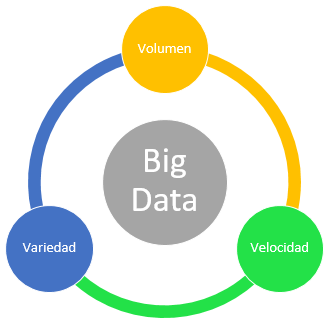
\includegraphics[width=.10\linewidth]{./marco_teorico/img/big_data_tres_v}
	\end{figure}

 				% Docker
 					%%%%%%%%%%%%%%%%%%%%%%%%%%%%%%%%%%%%%%%%%%%%%%%%%%%%%%%%%%%%%%%%%%%%%%%%%%%%%%%%%
%																				%
%	TRABAJO:	Trabajo Final													%
%				Especialidad en Ingenier�a en Sistemas de Informaci�n			%
%																				%
%		Titulo:																	%
%																				%
%		Autores:	Julian Nonino												%
%																				%
%	Capitulo sobre Docker														%	
%																				%
%	A�o: 2016																	%
%																				%
%%%%%%%%%%%%%%%%%%%%%%%%%%%%%%%%%%%%%%%%%%%%%%%%%%%%%%%%%%%%%%%%%%%%%%%%%%%%%%%%%

\chapter{Docker}

Docker es un proyecto de c�digo abierto que automatiza el despliegue de
aplicaciones dentro de contenedores de software, proporcionando una capa
adicional de abstracci�n y automatizaci�n de virtualizaci�n a nivel de sistema
operativo en Linux. Docker utiliza caracter�sticas de aislamiento de recursos
del kernel de Linux, tales como cgroups y espacios de nombres (namespaces) para
permitir que \emph{contenedores} independientes se ejecuten dentro de una sola
instancia de Linux, evitando la sobrecarga de iniciar y mantener m�quinas
virtuales. \cite{WikipediaDocker}

El soporte del kernel de Linux para los espacios de nombres a�sla de vista, en
su mayor�a, una aplicaci�n del entorno operativo, incluyendo �rboles de proceso,
red, ID de usuario y sistemas de archivos montados, mientras que los cgroups del
kernel proporcionan aislamiento de recursos, incluyendo la CPU, la memoria, el
bloque de E/S y de la red. Desde la versi�n 0.9, Docker incluye la librer�a
libcontainer como su propia manera de utilizar directamente las facilidades de
virtualizaci�n que ofrece el kernel de Linux, adem�s de utilizar las interfaces
abstra�das de virtualizaci�n mediante libvirt, LXC (Linux Containers) y
systemd-nspawn. \cite{WikipediaDocker}

Docker implementa una API de alto nivel para proporcionar contenedores livianos
que ejecutan procesos de manera aislada.
Construido sobre las facilidades proporcionadas por el kernel de Linux
(principalmente cgroups y namespaces), un contenedor Docker, a diferencia de una
m�quina virtual, no requiere incluir un sistema operativo independiente. En su
lugar, se basa en las funcionalidades del kernel y utiliza el aislamiento de
recursos (CPU, la memoria, el bloque E/S, red, etc.) y namespaces separados
para aislar de vista la aplicaci�n del sistema operativo. Docker accede a la
virtualizaci�n del kernel de Linux ya sea directamente a trav�s de la biblioteca
libcontainer (disponible desde Docker 0.9), o indirectamente a trav�s de
libvirt, LXC o systemd-nspawn. \cite{WikipediaDocker}

\begin{figure}[H]
	\centering
	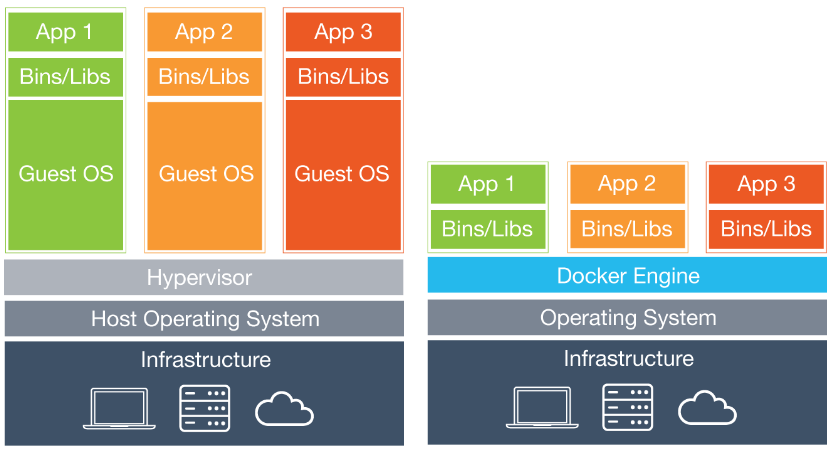
\includegraphics[width=1\linewidth]{./marco_teorico/img/vm-vs-docker}
	\caption{Contenedor Docker (derecha) versus M�quina Virtual (izquierda)
	\cite{WhatIsDocker2016}}
\end{figure}

Mediante el uso de contenedores, los recursos pueden ser aislados, los servicios
restringidos, y se otorga a los procesos la capacidad de tener una visi�n casi
completamente privada del sistema operativo con su propio identificador de
espacio de proceso, la estructura del sistema de archivos, y las interfaces de
red. Contenedores m�ltiples comparten el mismo n�cleo, pero cada contenedor
puede ser restringido a utilizar s�lo una cantidad definida de recursos como
CPU, memoria y E/S. \cite{WikipediaDocker}

Usando Docker para crear y gestionar contenedores puede simplificar la creaci�n
de sistemas altamente distribuidos, permitiendo m�ltiples aplicaciones, las
tareas de los trabajadores y otros procesos para funcionar de forma aut�noma en
una �nica m�quina f�sica o en varias m�quinas virtuales. Esto permite que el
despliegue de nodos se realice a medida que se dispone de recursos o cuando se
necesiten m�s nodos, lo que permite una plataforma como servicio (PaaS -
Plataform as a Service) de estilo de despliegue y ampliaci�n de los sistemas
como Apache Cassandra, MongoDB o Riak. Docker tambi�n simplifica la creaci�n y
el funcionamiento de las tareas de carga de trabajo o las colas y otros sistemas
distribuidos. \cite{WikipediaDocker}

\section{Imagenes y Contenedores}



\section{Docker Compose}

	Docker Compose es una herramienta que permite correr un sistema formado por
	m�ltiples contenedores.
	
	

 				% Apache Kafka
 					%%%%%%%%%%%%%%%%%%%%%%%%%%%%%%%%%%%%%%%%%%%%%%%%%%%%%%%%%%%%%%%%%%%%%%%%%%%%%%%%%
%																				%
%	TRABAJO:	Trabajo Final													%
%				Especialidad en Ingenier�a en Sistemas de Informaci�n			%
%																				%
%		Titulo:																	%
%																				%
%		Autores:	Julian Nonino												%
%																				%
%	Capitulo sobre Apache Kafka													%	
%																				%
%	A�o: 2016																	%
%																				%
%%%%%%%%%%%%%%%%%%%%%%%%%%%%%%%%%%%%%%%%%%%%%%%%%%%%%%%%%%%%%%%%%%%%%%%%%%%%%%%%%

\chapter{Apache Kafka}
				% Apache Storm
 					%%%%%%%%%%%%%%%%%%%%%%%%%%%%%%%%%%%%%%%%%%%%%%%%%%%%%%%%%%%%%%%%%%%%%%%%%%%%%%%%%
%																				%
%	TRABAJO:	Trabajo Final													%
%				Especialidad en Ingenier�a en Sistemas de Informaci�n			%
%																				%
%		Titulo:																	%
%																				%
%		Autores:	Julian Nonino												%
%																				%
%	Capitulo sobre Apache Storm													%	
%																				%
%	A�o: 2016																	%
%																				%
%%%%%%%%%%%%%%%%%%%%%%%%%%%%%%%%%%%%%%%%%%%%%%%%%%%%%%%%%%%%%%%%%%%%%%%%%%%%%%%%%

\chapter{Apache Storm}
\label{chapter_apache_storm}

Apache Storm es una herramienta de procesamiento de datos en tiempo real de
c�digo abierto y gratuita creada por Twitter y luego liberada en lo �rbita de
los proyectos Apache.

La finalidad de Storm es proveer un mecanismo confiable para procesamiento de
flujos de datos ilimitados, haciendo para flujos de datos (\emph{realtime
stream processing}) lo que Hadoop hace en procesamiento por lotes (\emph{batch
processing})\cite{ApacheStorm101}.

Deacuerdo a su documentaci�n, es capaz de procesar un mill�n de tuplas de datos
por segundo por nodo. Provee caracter�sticas de escalabilidad, tolerancia a
fallos, garant�as de que todos los datos ser�n procesados, etc�tera\cite{ApacheStorm101}.

Una \emph{topolog�a} de Storm consume flujos de datos, los procesa y genera
nuevos flujos de datos.

\section{Conceptos B�sicos}

	En �sta secci�n se analizar�n los conceptos b�sicos que definen a un programa
	Storm.
	
	\begin{figure}[H]
		\centering
		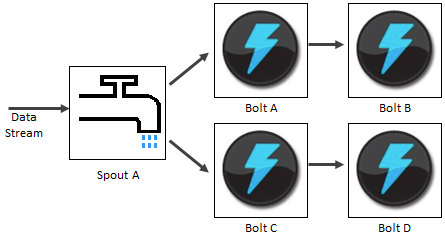
\includegraphics[width=.9\linewidth]{./marco_teorico/img/storm/topology}
	\end{figure}
	
	\subsection{\emph{Topologies} (Topolog�as)}
	
	Las \emph{topolog�as} son los contenedores de la l�gica de una aplicaci�n de
	procesamiento de datos en tiempo real. Es el an�logo a un trabajo de MapReduce
	de
	Hadoop\footnote{https://hadoop.apache.org/docs/current/hadoop-mapreduce-client/hadoop-mapreduce-client-core/MapReduceTutorial.html}.
	La diferencia principal con �stos �ltimos es que un trabajo MapReduce de
	Hadoop, eventualmente concluye mientras que las topolog�as pueden correr
	indefinidamente.
	Una topolog�a es un grafo formado por \emph{Spouts} y \emph{Bolts} conectados a
	trav�s de \emph{Stream Groupings}.
	
	\subsection{\emph{Streams} (Flujos de Datos)}
	
	\subsection{\emph{Spouts} (Tuber�as)}
	
	\subsection{\emph{Bolts} (Piezas))}

	\subsection{\emph{Streams Grouping} (Agrupamientos de Flujos de Datos)}
	
	\subsection{\emph{Tasks} (Tareas)}
	
	\subsection{\emph{Workers} (Trabajadores))}
	
 				% Apache Spark
 					%%%%%%%%%%%%%%%%%%%%%%%%%%%%%%%%%%%%%%%%%%%%%%%%%%%%%%%%%%%%%%%%%%%%%%%%%%%%%%%%%
%																				%
%	TRABAJO:	Trabajo Final													%
%				Especialidad en Ingenier�a en Sistemas de Informaci�n			%
%																				%
%		Titulo:																	%
%																				%
%		Autores:	Julian Nonino												%
%																				%
%	Capitulo sobre Apache Spark													%	
%																				%
%	A�o: 2016																	%
%																				%
%%%%%%%%%%%%%%%%%%%%%%%%%%%%%%%%%%%%%%%%%%%%%%%%%%%%%%%%%%%%%%%%%%%%%%%%%%%%%%%%%

\chapter{Apache Spark}

Spark es una herramienta de c�digo abierto desarrollada para procesar datos de
manera r�pida y f�cil. Su desarrollo comenz� en 2009 en el AMPLab de la
Universidad de Berkeley, siendo liberado su c�digo en 2010 como un proyecto
Apache.
Spark provee herramientas para procesar diversos conjuntos de datos de distinta
naturaleza (textos, grafos, etc�tera) y datos de distintas fuentes,
procesamiento de datos por lotes o procesamiento de un flujo de datos en tiempo
real.
Las aplicaciones para Spark pueden ser escritas en Java, Scala o Python y el
paquete incluye mas de 80 operadores de alto nivel para trabajar con los datos.
Adem�s de operaciones \emph{Map and Reduce} sobre Hadoop, soporta consultas SQL,
flujos de datos y \emph{Machine Learning} \cite{Penchikala2015SparkIntro}.
	
 				% Apache Flink
 					%%%%%%%%%%%%%%%%%%%%%%%%%%%%%%%%%%%%%%%%%%%%%%%%%%%%%%%%%%%%%%%%%%%%%%%%%%%%%%%%%
%																				%
%	TRABAJO:	Trabajo Final													%
%				Especialidad en Ingenier�a en Sistemas de Informaci�n			%
%																				%
%		Titulo:																	%
%																				%
%		Autores:	Julian Nonino												%
%																				%
%	Capitulo sobre Apache Flink													%	
%																				%
%	A�o: 2016																	%
%																				%
%%%%%%%%%%%%%%%%%%%%%%%%%%%%%%%%%%%%%%%%%%%%%%%%%%%%%%%%%%%%%%%%%%%%%%%%%%%%%%%%%

\chapter{Apache Flink}
\label{chapter_apache_flink}



\section{Conceptos\cite{ApacheFlink10Docs}}

	Los \emph{programas Flink} son programas comunes que implementan
	transformaciones en colecciones distribuidas, por ejemplo, filtrado,
	correspondencia, actualizaci�n de estado, uniones, agrupamientos, agregaciones,
	etc�tera. �stas colecciones se forman a partir de las fuentes de datos
	(\emph{sources}). Dichas fuentes se forman leyendo archivos, conectando Flink a
	un servidor de mensajes como Apache Kafka \ref{chapter_apache_kafka} o mediante
	colecciones definidas localmente.
	
	Los resultados de la ejecuci�n de un programa Flink son devueltos mediante el
	uso de receptores de datos \emph{sinks}. �stos receptores pueden consistir en
	escritura de archivos, impresi�n en la consola de ejecuci�n, etc�tera.
	
	Los programas Flink pueden correr localmente (standalone), embebidos en otros
	programas o en clusters.
	
	Dependiendo del tipo de fuente de datos (\emph{source}), es decir, acotados o
	no acotados, el programa Flink deber� realizar una ejecuci�n por lotes
	(\emph{batch}) o una ejecuci�n en tiempo real sobre el flujo de datos
	(\emph{straming}). Para el primer caso, se deber� utilizar la
	\textbf{\emph{DataSet API}} y para el segundo caso la \textbf{\emph{DataStream
	API}}.
	
	Los bloques b�sicos de un programa Flink son los flujos de datos (streams) y
	las transformaciones (operaciones).

	Al ejecutarse, un programa Flink se corresponde con lo que se conoce como
	\emph{Streaming Dataflow}. Cada \emph{Dataflow}, comienza con una o m�s fuentes
	de datos (\emph{sources}) y termina en uno o m�s receptores de datos
	(\emph{sinks}).
	En la mayor�a de los casos, existe una correspondencia uno a uno entre las
	transformaciones especificadas en el programa y las operaciones del
	\emph{Dataflow} pero puede ocurrir que una transformaci�n est� formada por mas
	de un operador de transformaci�n.
	
	\begin{figure}[H]
		\centering
		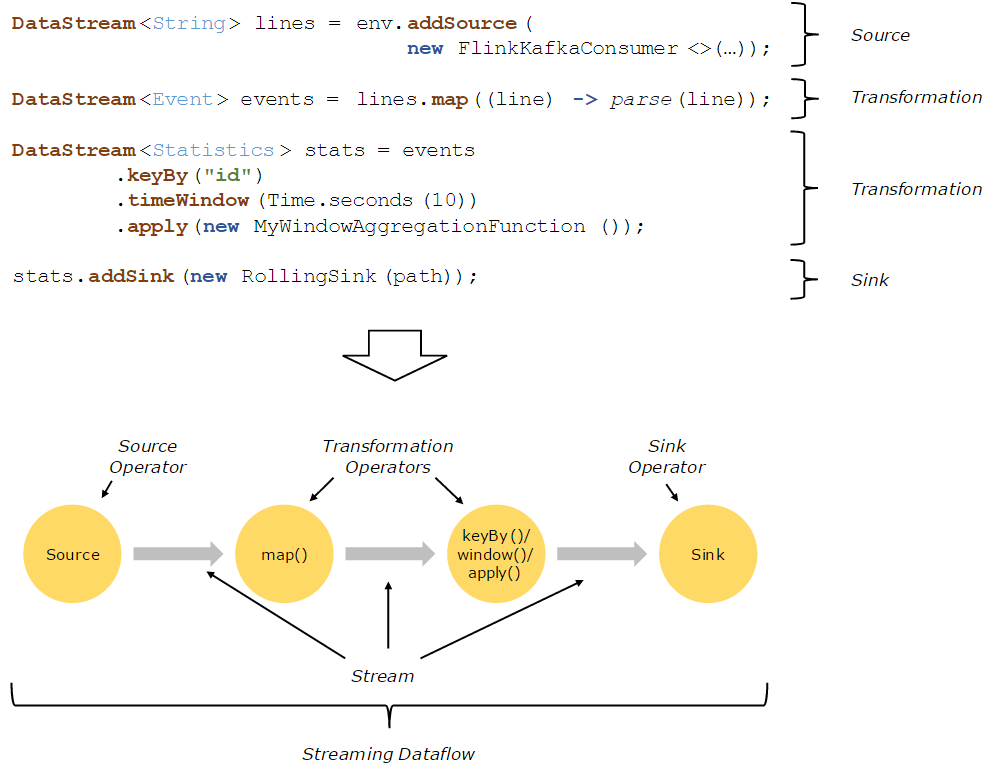
\includegraphics[width=1\linewidth]{./marco_teorico/img/flink/building_blocks}
		\caption{Bloques Fundamentales de un Programa Flink\cite{ApacheFlink10Docs}}
	\end{figure}

\subsection{Usar Flink}
	
		Para escribir un programa Flink, se deben incluir las libre�as Flink en el
		proyecto, en el caso de Maven, �sto se logra insertando las siguientes l�neas
		en el pom.xml del proyecto.
		
\lstset{language=XML}
\begin{lstlisting}
<dependency>
	<groupId>org.apache.flink</groupId>
	<artifactId>flink-core_2.11</artifactId>
	<version>1.0.3</version>
</dependency>
<dependency>
	<groupId>org.apache.flink</groupId>
	<artifactId>flink-java_2.11</artifactId>
	<version>1.0.3</version>
</dependency>
<dependency>
	<groupId>org.apache.flink</groupId>
	<artifactId>flink-clients_2.11</artifactId>
	<version>1.0.3</version>
</dependency>
<dependency>
	<groupId>org.apache.flink</groupId>
	<artifactId>flink-streaming-java_2.11</artifactId>
	<version>1.0.3</version>
</dependency>
<dependency>
	<groupId>org.apache.flink</groupId>
	<artifactId>flink-connector-kafka-0.9_2.11</artifactId>
	<version>1.0.3</version>
</dependency>
\end{lstlisting}
	
	\subsection{DataSet y DataStreams\cite{ApacheFlink10Docs}}		

		Para representar datos en un programa Flink existen dos tipos de clases
		DataSet y DataStream. Se puede considerar que son colecciones inmutables de
		datos que pueden contener duplicados. En el caso del DataSet la cantidad de
		datos es finita, mientras que en un DataStream pueden ser ilimitados.
		
		�stas colecciones son diferentes a las Java en el sentido de que son
		inmutables, una vez creadas no pueden a�adirse ni removerse elementos. Tampoco
		es posible inspeccionar los elementos contenidos dentro de la colecci�n.
		
		Como se menciono anteriormente, una colecci�n DataSet o DataStream es creada
		en el momento en que se a�ade una fuente de datos \emph{source} y nuevas
		colecciones son creadas cada vez que una operaci�n de transformaci�n es
		ejecutada.

	\subsection{Evaluaci�n Postergada}
	
		Al ejecutar un programa Flink, el m�todo \emph{main} es ejecutado pero la
		carga de datos y las transformaciones no ocurren directamente. Cada operaci�n
		es creada y a�adida a un plan de ejecuci�n del programa. Las operaciones, son
		ejecutadas cuando son exlicitamente disparada mediante el llamado del m�todo
		\emph{execute()} sobre el entorno de ejecuci�n \cite{ApacheFlink10Docs}.
	

Flink DataStream API Programming Guide (Source: https://ci.apache.org/projects/flink/flink-docs-release-1.0/apis/streaming/index.html)

DataStream programs in Flink are regular programs that implement transformations
on data streams (e.g., filtering, updating state, defining windows,
aggregating). The data streams are initially created from various sources (e.g.,
message queues, socket streams, files). Results are returned via sinks, which
may for example write the data to files, or to standard output (for example the
command line terminal). Flink programs run in a variety of contexts, standalone,
or embedded in other programs. The execution can happen in a local JVM, or on
clusters of many machines.


 		% Desarrollo
 			\part{Desarrollo}
 				% Desarrollo e Implementaci�n
 					%\input{./desarrollo/diseno_implementacion/chap_diseno_implementacion}
 				% Implementaci�n en FPGA
 					%\input{./desarrollo/implementacion_FPGA/chap_implementacion_fpga}
 		% Resultados y Conclusiones			
 			\part{Resultados y Conclusiones}
 				%Resultados obtenidos
 					%\input{./conclusiones/resultados/chap_resultados}
 				% Conclusiones
 					%%%%%%%%%%%%%%%%%%%%%%%%%%%%%%%%%%%%%%%%%%%%%%%%%%%%%%%%%%%%%%%%%%%%%%%%%%%%%%%%%
%																				%
%	TRABAJO:	Trabajo Final													%
%				Especialidad en Ingenier�a en Sistemas de Informaci�n			%
%																				%
%		Titulo:																	%
%																				%
%		Autores:	Julian Nonino												%
%																				%
%	Conclusiones																%	
%																				%
%	A�o: 2016																	%
%																				%
%%%%%%%%%%%%%%%%%%%%%%%%%%%%%%%%%%%%%%%%%%%%%%%%%%%%%%%%%%%%%%%%%%%%%%%%%%%%%%%%%

\chapter{Conclusiones}









https://www.infoq.com/articles/stream-processing-hadoop
Conclusion \cite{Wahner2014}

Stream processing is required when data has to be processed fast and / or
continuously, i.e. reactions have to be computed and initiated in real time.
This requirement is coming more and more into every vertical. Many different
frameworks and products are available on the market already, however the number
of mature solutions with good tools and commercial support is small today.
Apache Storm is a good, open source framework; however custom coding is required
due to a lack of development tools and there is no commercial support right now.
Products such as IBM InfoSphere Streams or TIBCO StreamBase offer complete
products, which close this gap. You definitely have to try out the different
products, as the websites do not show you how they differ regarding ease of use,
rapid development and debugging, and real-time streaming analytics and
monitoring. Stream processing complements other technologies such as a DWH and
Hadoop in a big data architecture - this is not an "either/or" question. Stream
processing has a great future and will become very important for most companies.
Big Data and Internet of Things are huge drivers of change.

 				% Trabajo futuro
 					%%%%%%%%%%%%%%%%%%%%%%%%%%%%%%%%%%%%%%%%%%%%%%%%%%%%%%%%%%%%%%%%%%%%%%%%%%%%%%%%%
%																				%
%	TRABAJO:	Trabajo Final													%
%				Especialidad en Ingenier�a en Sistemas de Informaci�n			%
%																				%
%		Titulo:																	%
%																				%
%		Autores:	Julian Nonino												%
%																				%
%	Trabajo Futuro																%	
%																				%
%	A�o: 2016																	%
%																				%
%%%%%%%%%%%%%%%%%%%%%%%%%%%%%%%%%%%%%%%%%%%%%%%%%%%%%%%%%%%%%%%%%%%%%%%%%%%%%%%%%

\chapter{Trabajo Futuro}	
 	
	% APENDICES
		\appendix
		\part{Ap�ndices}
		
			% Nuevo proyecto en Xilinx XPS
				%\input{./apendices/nuevos_proyectos_XPS/nuevos_proyectos_XPS}
			% Creacion de un nuevo IP core	
				%\input{./apendices/creacion_IP_core/creacion_IP_core}
			% Interrupciones en los IP core
				%\input{./apendices/interrupciones/interrupciones}
			% Gesti�n de la metodolog�a de desarrollo
				%%%%%%%%%%%%%%%%%%%%%%%%%%%%%%%%%%%%%%
%									%
%	Copyright 2014 - Julian Nonino	%								
%									%
%%%%%%%%%%%%%%%%%%%%%%%%%%%%%%%%%%%%%

\section{Metodolog�a de desarrollo}

	El supuesto de �sta tesis consiste en que es posible dise�ar e implementar un
	herramienta de ense�anza en l�nea que permita a los estudiantes relacionar
	t�cnicas de estimaci�n y planeamiento utilizadas en Scrum con pr�cticas
	tradicionales de estimaci�n utilizando planeamiento de escenarios y generaci�n
	autom�tica de datos para pron�stico.

	Basado en el supuesto anterior, la primera etapa de la tesis consistir� en la
	recolecci�n y an�lisis de material sobre el tema. Se buscar�n libros, art�culos
	y presentaciones de congresos y conferencias, \emph{white papers}, art�culos de
	revistas especializadas, adem�s de blog, sitios de noticias, foros, de opini�n,
	etc�tera.

	Los puntos m�s importantes para la realizaci�n de la Revisi�n Sistem�tica de la
	Literatura son:
	\begin{itemize}
		\item Metodolog�as �giles (Agile). 
		\item Scrum.
		\item Pr�cticas de estimaci�n y planeamiento en Scrum.
		\item Herramientas existentes para soporte de los procesos de estimaci�n y
		planeamiento en Scrum.
		\item Historias de usuario, puntos de historia, horas ideales, velocidad.
		\item Proyectos de alcance fijo, duraci�n fija o precio fijo.
		\item Estimaci�n y planeamiento para m�ltiples equipos en Scrum.
		\item Simulaci�n de Monte Carlo.
		\item Simulaci�n de escenarios alternativos.
		\item Ense�anza de las pr�cticas de estimaci�n y planeamiento utilizadas en
		Scrum a alumnos de novel universitario.
	\end{itemize}

	Analizada la bibliograf�a, se deber�n determinar los requerimientos de la
	herramienta y se deber� elaborar un dise�o que contemple las pr�cticas de
	estimaci�n y planeamiento utilizadas en Scrum, combinadas con pr�cticas
	avanzadas pensando en el �mbito universitario, profesores y alumnos, como
	destinatario de la herramienta.

	Luego, se comenzar� la construcci�n del primer prototipo de la herramienta en
	Microsoft Excel pensando la simplicidad de uso de la misma y en la claridad de
	los conceptos utilizados para que sea �til en el �mbito universitario. Dicha
	herramienta podr�a ser probada por alumnos durante los cursos de Ingenier�a de
	Software y Gesti�n de la Calidad del Software pertenecientes a la carrera
	Ingenier�a en Computaci�n de la Universidad Nacional de C�rdoba. Se deber�n
	definir m�tricas para la evaluaci�n del impacto que produzca la herramienta
	sobre los alumnos e identificar falencias, errores y mejoras para continuar el
	desarrollo.
	
	Los resultados obtenidos deber�n ser analizados detenidamente con el fin de
	identificar posibles correcciones y mejoras en los requerimientos y dise�os
	originales, considerando que la herramienta deber� ser desarrollada como
	aplicaci�n web disponible en l�nea.

	Corregidos y mejorados los requerimientos originales e identificados nuevos
	requerimientos y conceptos que deben ser implementados en la segunda versi�n de
	la herramienta, se comenzar� con la construcci�n de la misma.
	
	Para comenzar con �sta etapa se deben analizar las distintas alternativas en
	lenguajes de programaci�n, frameworks y otras herramientas utilizadas en el
	mercado para el desarrollo de aplicaciones web. Adem�s, se deben analizar
	alternativas para hacer que la aplicaci�n web desarrollada pueda ser puesta en
	l�nea.
	
	Estando construida la herramienta, puede ser probada nuevamente en el �mbito
	universitario, como se mencion� anteriormente. Dicha prueba generar� resultados
	y estad�sticas de uso, ser�n encontrados errores y mejoras y, ser�n
	identificados fortalezas y beneficios generados por la existencia de la
	herramienta. Los datos recolectados ser�n analizados, contrastados con la
	hip�tesis y objetivos planteados al comienzo del desarrollo y luego plasmados
	en el informe de tesis con las respectivas conclusiones.
	
	\newpage

			% C�digos en Verilog de los IP cores
				%\input{./apendices/codigos_ipcores/codigos_ipcores}
			% C�digos en C de los programas ejecutados
				%\input{./apendices/codigos_programas/codigos_programas}
	
	%INICIO DE LA PARTE FINAL. Bibliografia e �ndices
		\backmatter
		% Referencias
			\addcontentsline{toc}{chapter}{Bibliograf�a}
			\printbibliography
		% Indices
			% Indice de contenido
				\addcontentsline{toc}{chapter}{�ndice de contenido}
				\tableofcontents
			% �ndice de Figuras
				\cleardoublepage
				\addcontentsline{toc}{chapter}{�ndice de Figuras}
				\listoffigures

\end{document}
